\section{Paradigm Shift}

The Transformer architecture is pervasive in modern natural language processing. First introduced by Vaswani et al. \cite{DBLP:journals/corr/VaswaniSPUJGKP17}, it was originally applied to the sequence-to-sequence problem in language translation. The mapping from $X \in \mathbb{R}^{n \times d}$ to $Y \in \mathbb{R}^{n \times d}$ is complex, as the mapping of each individual element $x_i$ in the sequence must account for the entire context window $X$.

\vskip 0.2in

This problem arises in natural language processing, where mapping between sequence domains is common in tasks like machine translation (mapping between two different languages) or text summarization (mapping from an ‘expanded’ version to a more ‘condensed’ one within the same language). The concept has also been extended to other fields, such as image understanding, and has enabled cross-domain applications like text-to-image or image-to-text generation, demonstrating the versatility and universal applicability of the architecture.

\vskip 0.2in

To address the challenge of context-dependent, cross-domain mapping, Transformers utilize multiple \textbf{attention blocks} designed to learn context-aware mappings. Three projection matrices, $W^Q$, $W^K$, and $W^V$, are learned. When multiplied with the input $X$, they yield $Q$, $K$, and $V$, respectively. These tensors function as a differentiable lookup table: the key vector $k_i$ is multiplied by the query vectors $q_i$ at all positions to determine the relevance of other positions for position $i$. The $V$ matrix then uses the attention scores to compute the final embedding $Z$ of $X$.

\begin{figure}[h]
\[ Z = softmax(\frac{QK^T}{\sqrt{d_k}})VW^O \text{, where } Q = XW^Q\text{, }K = XW^K\text{, } V = XW^V \]
\caption[Attention Equation]{The attention equation. The softmax function is used to map attention scores at each position to a probability distribution. Scaling by the size of the key vectors, $d_k$, is applied to normalize these values. A final linear layer, $W^O$, is applied to the computed attention vectors, resulting in the final latent representation.}
\end{figure}

\vskip 0.2in

Transformers divide their architecture into two main components: the encoder and the decoder. Each section consists of multiple stacked attention layers to create more powerful mappings. However, the authors introduce two key modifications in the decoder. First, the encoder’s output is treated as a universal latent representation of the input, so the decoder layers project $W^Q$ onto the final encoder output, $Z^{e}$, instead of using the decoder’s input vectors. Second, since the decoder generates sequences one step at a time, using the context $\overline{i+1..n}$ to compute the current position $i$ would be incorrect. To address this, future positions are masked during training. Finally, the output of the last attention layer in the decoder is passed through a classification head to generate the desired sequence $Y$.

\begin{figure}[h]
\[ Z^d = softmax(\frac{QK^T + M}{\sqrt{d_k}})VW^O \text{, where } Q = Z^eW^Q\text{, }K = XW^K\text{, } V = XW^V \]
\caption[Decoder Modification in Transformer Architecture]{The three linear layers in attention reformulated with decoder constraints. Here, $X$ represents the output of the previous attention layer in the decoder. $M$ is a mask applied over the attention filter to block future values by adding a “negative infinity” value below the second diagonal. This modification is referred to as cross-attention in the literature, distinguishing it from the encoder’s ‘self-attention’ mechanism.}
\end{figure}

At their core, Transformers build upon several foundational concepts in deep learning. Convolutional neural networks (CNNs) create context-aware representations using a smaller sliding window to downscale high-dimensional vectors, particularly in image processing. Recurrent neural networks (RNNs) similarly aim to capture context-aware embeddings by computing position $i$’s embedding based on state embeddings that encode previous positions (or, in some variants, both past and future windows). Earlier architectures, like U-NET by Ronneberger et al. \cite{ronneberger2015unetconvolutionalnetworksbiomedical}, also employed latent representations to map from one domain to another. However, Transformers surpass these models by utilizing the full context of the sequence at all times and introducing a simplified architecture that enables highly parallel computation, unlike the sequential backpropagation through time used in RNNs.

\pskip

From the perspective of an \gls{nlp} practitioner at the start of this decade, Transformers represented an incremental improvement in the deep learning paradigm, rather than a revolutionary shift. Yet, this same architecture has since sparked debates about the potential for general artificial intelligence \cite{bubeck2023sparksartificialgeneralintelligence}. OpenAI’s \gls{gpt} family of language models builds on the Transformer architecture, specifically using its decoder to generate text continuations from word embeddings based on user input. Unlike traditional language models, \gls{gpt} models are trained on vast text corpora, with parameter counts several orders of magnitude larger. This difference in scale involves hundreds of gigabytes of training data, sourced from web crawls, and models with hundreds of billions of parameters.

\pskip

Beginning with the GPT-3 iteration, the model demonstrated emergent and unexpected behaviors. Unlike traditional models, which are typically trained for a single task using one or more closely related datasets, GPT-3 exhibited few-shot and even zero-shot capabilities. With zero or only a few examples provided in the prompt, the model could perform at a level comparable to state-of-the-art models on diverse, unrelated tasks, including question answering, basic arithmetic, reasoning, translation, and summarization.

\begin{figure}[h!]
    \centering
    \captionsetup{format=plain, font=small, labelfont=bf}
    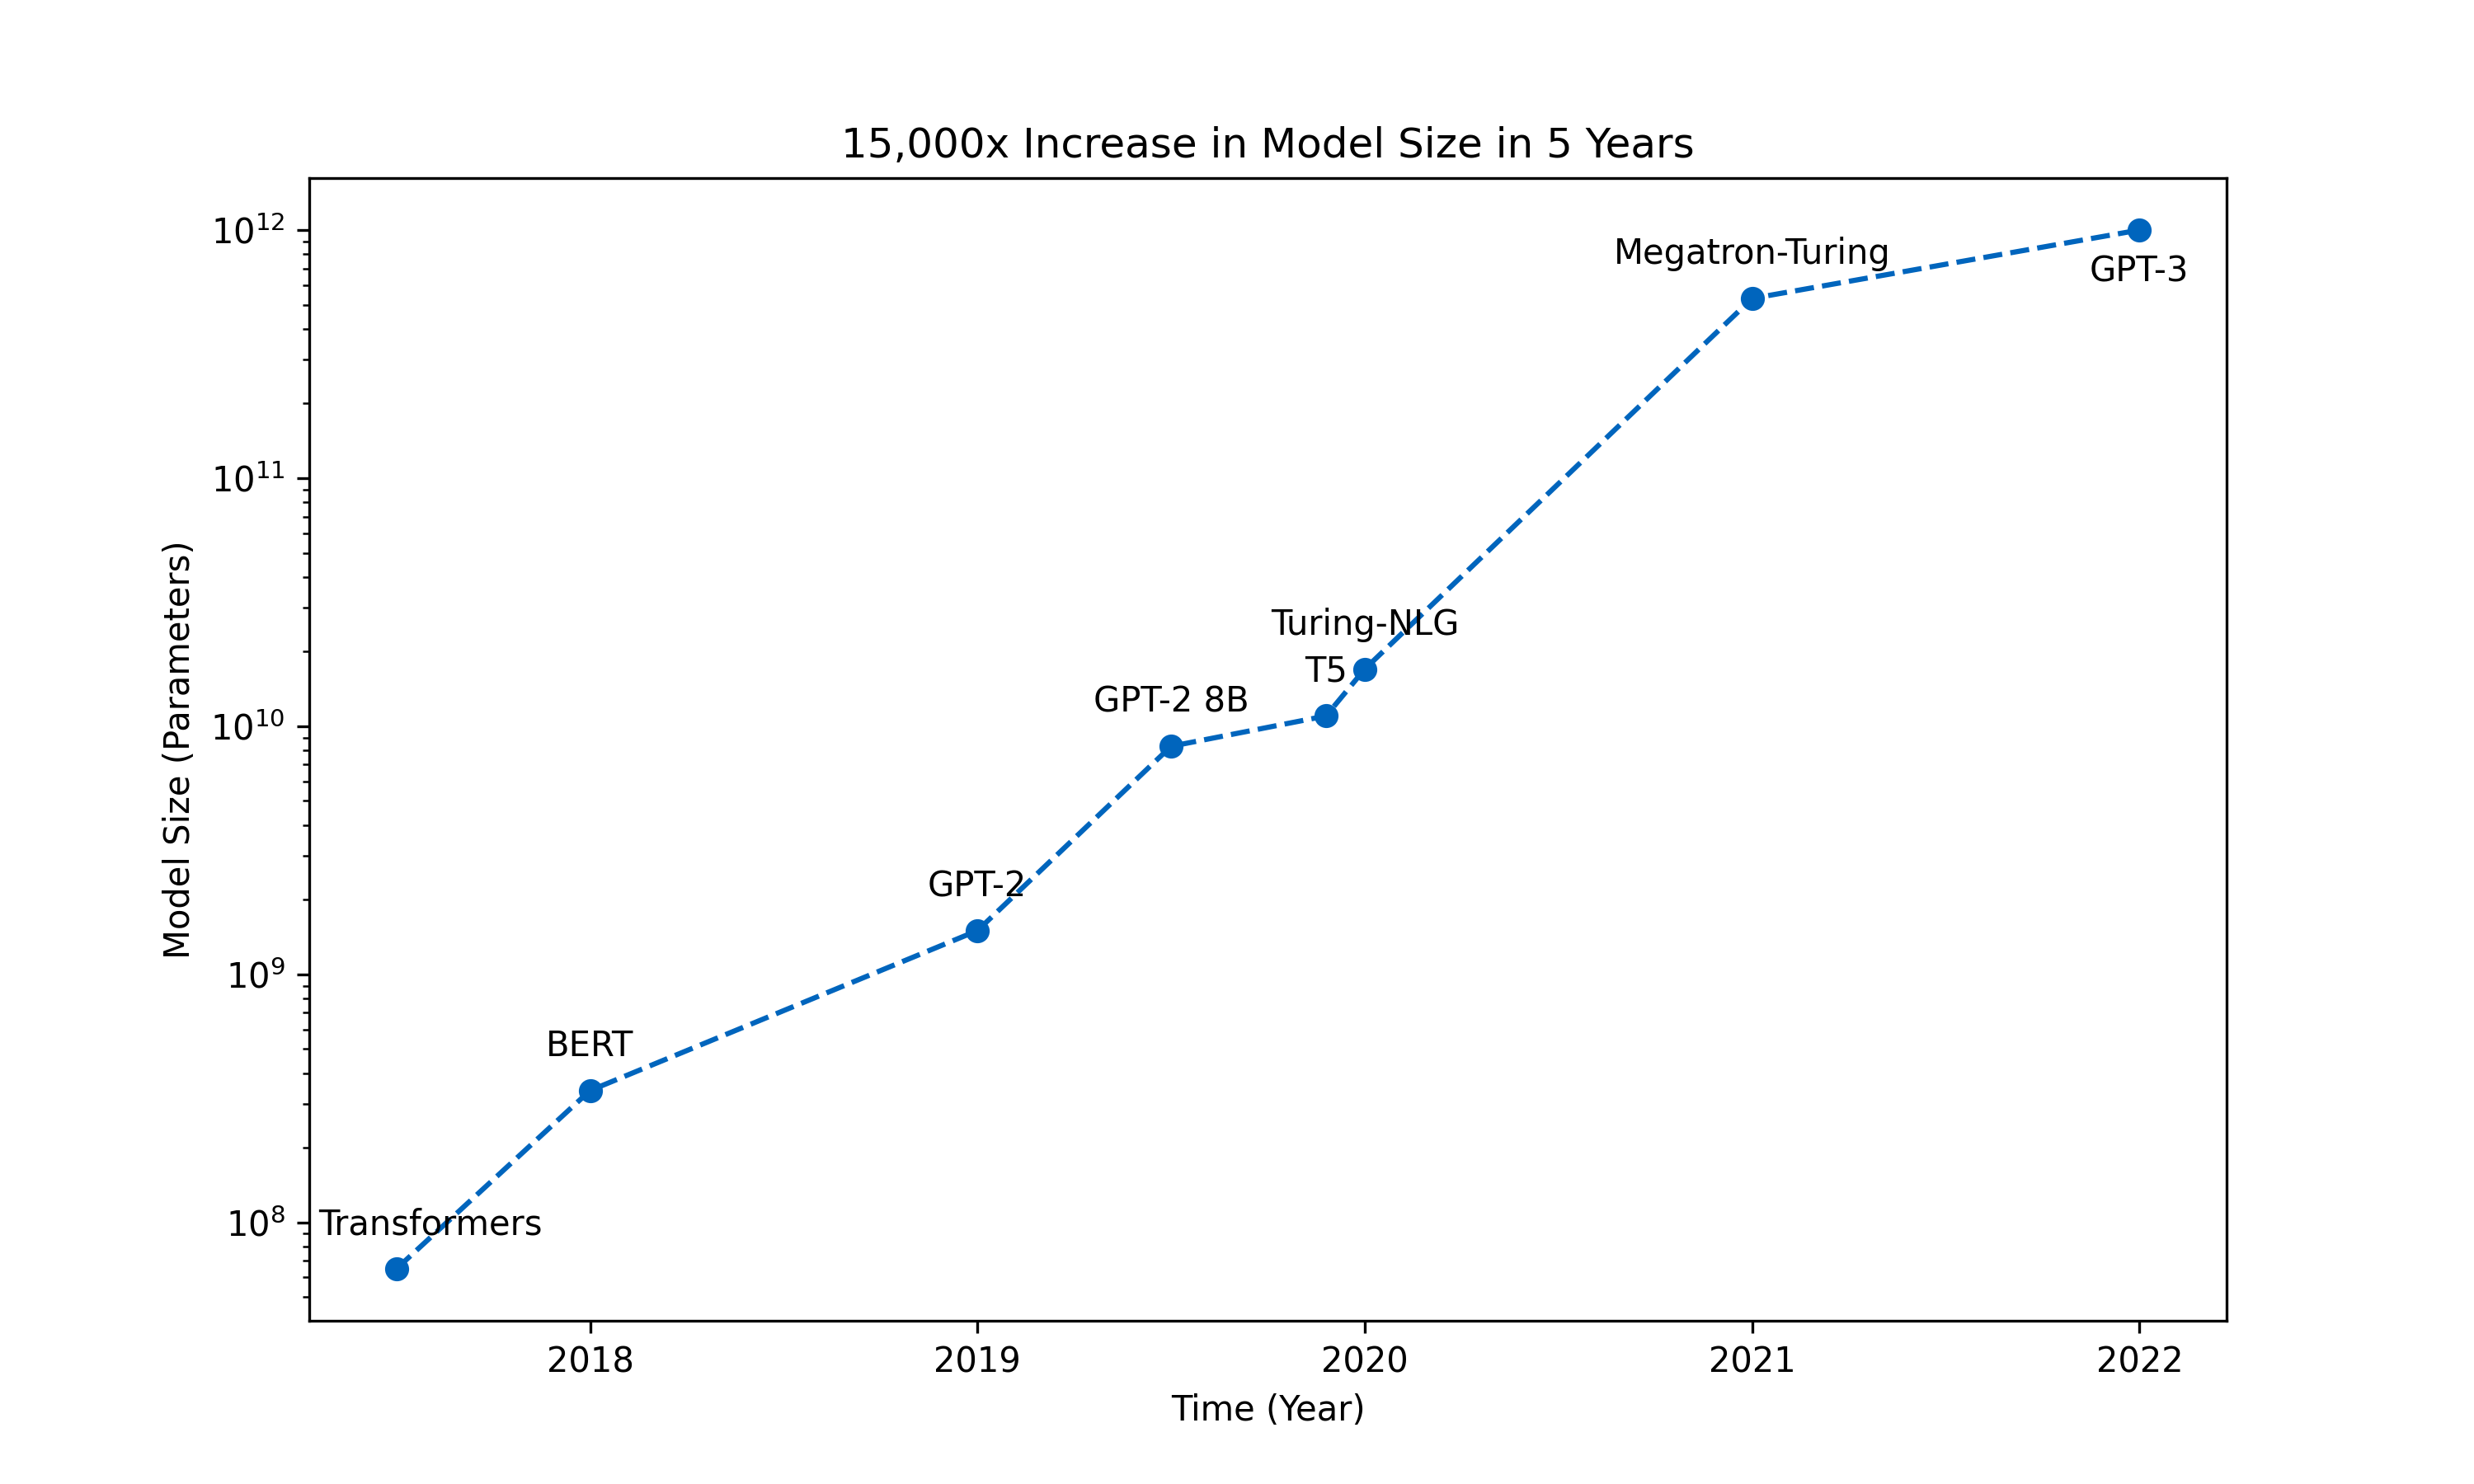
\includegraphics[width=\linewidth]{figures/modelsizeincrease.png}
    \caption[Progression of Models Size in \glspl{llm}]{The exponential increase in the number of parameters in \glspl{llm} is the main cause of their few-shot capabilities.}
    \label{fig:sample_plot}
\end{figure}

Such behavior has been previously observed to some extent within the field of meta-learning. Meta-learning aims to create meta-objectives for optimization, such as using meta-models trained on related but distinct tasks—like training the same machine translation model on multiple language pairs to enhance generalization with fewer examples. Some approaches explore meta-objectives by introducing penalties for using large training datasets, encouraging the discovery of parameter configurations that can be fine-tuned with minimal data on new tasks. Additionally, meta-optimizers are studied to fine-tune optimizers for more efficient training across families of functions \cite{metalearning}.

\pskip

While these methods have led to improved generalization, they also introduce complex training procedures involving second-order optimizations. Moreover, they require significant expert involvement \cite{Yao2018TakingHO}, and some argue that they merely shift the problem of distribution mismatch \cite{wiles2021finegrainedanalysisdistributionshift}, as models can still be applied to data distributions that differ from those seen during training.

\pskip

Given the challenges and extensive human effort invested in improving individual models, the prospect of training a single model and applying it across all tasks naturally garnered the attention of the scientific community. This has led to large language models (LLMs) being referred to as \glspl{fm} (foundational models) \cite{foundationalmodels}. The power and versatility of these models have also attracted interest from fields such as psychology and human-computer interaction. Surveys analyzing social media posts reveal public curiosity about these models, with users testing complex, human-like behaviors such as humor and irony while exploring the models’ capabilities \cite{Dynel2023}.

\pskip

In writing tasks, LLMs are increasingly used in both academic and practical contexts, such as emails or letters. Users’ ‘cognitive appreciation’—the recognition of the model’s utility—often surpasses their initial ‘emotional appreciation’ for its human-like interactions. However, while users tend to view these models positively as assistants, they remain cautious about the accuracy of the information provided \cite{Luther2024} \cite{XinXiaCao2023} \cite{Herbold2023}.

\pskip

Human intelligence is often defined by the ability to learn and apply previously acquired knowledge to new tasks \cite{Sternberg2012}. By this definition, \glspl{llm} could be considered intelligent, as they can process new information and accomplish goals. However, the nature of this intelligence differs fundamentally from human intelligence. \glspl{llm} are stochastic models that predict and output the next most likely word based on the given context, similar in principle to \gls{ngram} models \cite{brown1992class}.